\chapter{Linear Geometry}
\label{chap:linear-geometry}

This chapter is dedicated to fostering a geometric intuition about
\hyperref[def:vector]{vectors} as introduced in
\myref{section}{sec:describing-solution-sets-of-linear-systems}. There, we used
them as a convenient way of grouping data. They, however, are also apt
representations of a geometric concept -- the concept of a `shift in space'.

Before we move on, though, we need elucidate what we mean by `geometry' and
`space'. The former word has a widespread connotation of `drawing stuff using a
ruler and a compass on a sheet of paper'. This is hardly the \emph{geometry} we
have in mind in this text. Although circles, lines and triangles are geometric
objects to us as well, the fundamental notion of geometry, which is scarcely
properly discussed in high-school setting, is \emph{space}.

\emph{Space} is the `place where we do geometry', in essence. We begin by
arguing the most intuitive way of describing space is that of a set of
dimensions (or directions of movement) where each dimension is a
\emph{continuum}, meaning, in whichever direction I move, there are no holes
along the way. We trust the first \emph{continuum} (a `set without holes') dear
readers encountered, are the real numbers, $\R$. They seem a good candidate for
the definition of space.

Firstly, we define the \emph{one-dimensional} space to be exactly $\R$. You
might wonder how this makes any sense. Well, a space with just one dimension is
an infinite line like below.
\begin{center}
 \begin{tikzpicture}
  \draw[arrows={Latex[width=6pt,length=8pt]-Latex[width=6pt,length=8pt]}]
   (0,0) to (10,0);
 \end{tikzpicture}
\end{center}
How is this related to $\R$? Quite trivially. Pick any point on the line and
label it $0$. Then pick yet another different point and label it $1$. Like so.
\begin{center}
 \begin{tikzpicture}
  \draw[arrows={Latex[width=6pt,length=8pt]-Latex[width=6pt,length=8pt]}]
   (0,0) to (10,0);
  \draw[thick,BrickRed] (5,0.1) -- (5,-0.1);
  \node[BrickRed] at (5,-0.4) {$0$};
  \draw[thick,RoyalBlue] (6,0.1) -- (6,-0.1);
  \node[RoyalBlue] at (6,-0.4) {$1$};
 \end{tikzpicture}
\end{center}
Just like that, we have forged a \emph{correspondence} between an infinite line
and the real numbers. Any real number $r \in \R$ corresponds to the point on the
line distant exactly $|r|$ from $0$ -- to the right if it's positive, and to the
left if it's negative. For example, the number $\clg{-3.14}$ is represented as
the following \clg{point}.
\begin{center}
 \begin{tikzpicture}
  \draw[arrows={Latex[width=6pt,length=8pt]-Latex[width=6pt,length=8pt]}]
   (0,0) to (10,0);
  \draw[thick,BrickRed] (5,0.1) -- (5,-0.1);
  \node[BrickRed] at (5,-0.4) {$0$};
  \draw[thick,RoyalBlue] (6,0.1) -- (6,-0.1);
  \node[RoyalBlue] at (6,-0.4) {$1$};
  \node[ForestGreen] at (1.86,-0.4) {$-3.14$};
  \draw[thick,ForestGreen] (1.86,0.1) -- (1.86,-0.1);
  \draw[decorate,decoration={brace,raise=5pt,amplitude=8pt}] (1.86,0) -- (5,0);
  \node at (3.43,0.7) {$3.14$};
 \end{tikzpicture}
\end{center}

Why stop at one dimension? We may add as many dimensions as we like by simply
inventing new directions of movement. Knowing that one direction of movement
amounts to the set of real numbers, we get as many directions as we choose to
include copies of the set of real numbers.

To make the preceding paragraph more tangible, let's first add a second
dimension, which we typically depict as another line perpendicular to the first
one and meeting it at $0$. Like this.
\begin{center}
 \begin{tikzpicture}
  \draw[arrows={Latex[width=4pt,length=6pt]-Latex[width=4pt,length=6pt]}]
   (0,0) to (4,0);
  \draw[arrows={Latex[width=4pt,length=6pt]-Latex[width=4pt,length=6pt]}]
   (2,2) to (2,-2);
  \draw[thick,BrickRed] (2,0.1) -- (2,-0.1);
  \draw[thick,BrickRed] (2.1,0) -- (1.9,0);
  \node[BrickRed] at (1.7,-0.3) {$0$};
  \draw[thick,RoyalBlue] (3,0.1) -- (3,-0.1);
  \node[RoyalBlue] at (3,-0.3) {$1$};
  \draw[thick,RoyalBlue] (1.9,1) -- (2.1,1);
  \node[RoyalBlue] at (1.7,1) {$1$};
 \end{tikzpicture}
\end{center}
Now, we have the entire \emph{plane} to move about. We are free to tread as far
right (or left) as we wish and as far up (or down) as we wish. Therefore, each
point here is given two numbers -- one on the axis of horizontal movement and
one on the axis of vertical movement.
\begin{center}
 \begin{tikzpicture}
  \draw[arrows={Latex[width=4pt,length=6pt]-Latex[width=4pt,length=6pt]}]
   (0,0) to (4,0);
  \draw[arrows={Latex[width=4pt,length=6pt]-Latex[width=4pt,length=6pt]}]
   (2,2) to (2,-2);
  \draw[thick,BrickRed] (2,0.1) -- (2,-0.1);
  \draw[thick,BrickRed] (2.1,0) -- (1.9,0);
  \node[BrickRed] at (1.7,-0.3) {$0$};
  \draw[thick,RoyalBlue] (3,0.1) -- (3,-0.1);
  \node[RoyalBlue] at (3,-0.3) {$1$};
  \draw[thick,RoyalBlue] (1.9,1) -- (2.1,1);
  \node[RoyalBlue] at (1.7,1) {$1$};
  \draw[thick,RoyalBlue] (1.9,1) -- (2.1,1);
  \node[ForestGreen] at (1.55,0.6) {$0.6$};
  \draw[thick,ForestGreen] (1.9,0.6) -- (2.1,0.6);
  \draw[thick,ForestGreen] (3.5,0.1) -- (3.5,-0.1);
  \node[ForestGreen] at (3.5,-0.3) {$1.5$};
  
  \draw[ForestGreen,dashed] (3.5,0) -- (3.5,0.6);
  \draw[ForestGreen,dashed] (2,0.6) -- (3.5,0.6);
  \node[ForestGreen,circle,fill,inner sep=1.5pt] at (3.5,0.6) {};
  \node[ForestGreen] at (4.3,0.9) {$(1.5,0.6)$};
 \end{tikzpicture}
\end{center}
We call the set of all ordered pairs of real numbers the \emph{cartesian
product} of real numbers with themselves and denote it $\R \times \R$ (or $\R^2$
for short). Hence, the two-dimensional space (also called \emph{plane}) is just
equivalent to $\R^2$.

We needn't stop at two dimensions. As stated before, we may add as many
directions of movement as desired. The preceding small examples justify the
following definition.

\begin{definition}{Space}{space}
 We call the set $\R^{n}$ of all (ordered) $n$-tuples of real numbers the
 \emph{$n$-dimensional (real) space}. 
\end{definition}

We claimed that a \emph{vector} represents a shift in space. We now make that
idea precise. Consider the points $(a_1,a_2)$ and $(b_1,b_2)$ in $\R^2$. There
exists a straight path from one to the other. The trajectory of such path can be
represented as a pair of numbers where the first one signifies the distance we
are to travel horizontally to reach $b_1$ from $a_1$ and the second number the
vertical distance from $a_2$ to $b_2$. Clearly, the first distance equals $b_1 -
a_1$ and the second $b_2 - a_2$. We can collect these numbers into the vector
\[
 \mathbf{v} = 
 \begin{pmatrix}
  b_1 - a_1\\
  b_2 - a_2
 \end{pmatrix}
\]
which now serves as a representation of the \emph{movement} or \emph{shift} from
the point $(a_1,a_2)$ to the point $(b_1,b_2$). In this scenario, we call
$(a_1,a_2)$ the \emph{root} or \emph{source} of the vector $\mathbf{v}$ and the
point $(b_1,b_2)$ its \emph{end} or \emph{target}.

Naturally, this idea is easily scaled to higher dimensions. Given points
\begin{align*}
 a &= (a_1,a_2,\ldots,a_n),\\
 b &= (b_1,b_2,\ldots,b_n)
\end{align*}
in $\R^{n}$, the vector with \emph{source} $a$ and \emph{target} $b$ is exactly
\[
 \begin{pmatrix}
  b_1 - a_1\\
  b_2 - a_2\\
  \vdots\\
  b_n - a_n
 \end{pmatrix}.
\]
\begin{figure}[ht]
 \centering
 \begin{tikzpicture}
  \tkzInit[xmin=-1,xmax=4,ymin=-1,ymax=4]
  \tkzDrawX[arrows={-Latex[width=4pt,length=6pt]},label=]
  \tkzDrawY[arrows={-Latex[width=4pt,length=6pt]},label=]
  \tkzDefPoints{1/2/a,3/3/b,1/0/a1,0/2/a2,3/0/b1,0/3/b2}
  \tkzDrawPoints[size=4,fill=black](a1,a2,b1,b2)
  \tkzLabelPoint[below=1mm](a1){$1$}
  \tkzLabelPoint[below=1mm](b1){$3$}
  \tkzLabelPoint[left=1mm](a2){$2$}
  \tkzLabelPoint[left=1mm](b2){$3$}

  \tkzDrawSegment[-Latex,thick,Fuchsia,shorten <=4pt,shorten >=4pt](a,b)
  \tkzLabelSegment[pos=0.5,below,Fuchsia](a,b){$\mathbf{v}$}
  \tkzDrawSegments[dashed](a1,a a2,a b1,b b2,b)
  \tkzDrawPoints[size=6,BrickRed,fill=BrickRed](a,b)
 \end{tikzpicture}
 \caption{Depiction of a vector $\clm{\mathbf{v}}$ with source $\clr{(1,2)}$ and
 target $\clr{(3,3)}$.}
 \label{fig:vector}
\end{figure}

Observe how this idea of vector being a \emph{shift} sings in unison with the
definitions of \hyperref[def:adding-vectors]{vector addition} and
\hyperref[def:multiplying-vector-by-a-number]{scalar multiplication}. The sum of
the vector of source $a$ and target $b$ with the vector of source $b$ and target
$c$ is the vector of source $a$ and target $c$ (cf.
\myref{figure}{fig:vector-addition}). This is testified by the simple
calculation
\[
 \begin{pmatrix}
  b_1 - a_1\\
  b_2 - a_2\\
  \vdots\\
  b_n - a_n
 \end{pmatrix}
 + 
 \begin{pmatrix}
  c_1 - b_1\\
  c_2 - b_2\\
  \vdots\\
  c_n - b_n
 \end{pmatrix}
 =
 \begin{pmatrix}
  b_1 - a_1 + c_1 - b_1\\
  b_2 - a_2 + c_2 - b_2\\
  \vdots\\
  b_n - a_n + c_n - b_n
 \end{pmatrix}
 = 
 \begin{pmatrix}
  c_1 - a_1\\
  c_2 - a_2\\
  \vdots\\
  c_n - a_n
 \end{pmatrix}
\]
for points $(a_1,\ldots,a_n), (b_1,\ldots,b_n)$ and $(c_1,\ldots,c_n)$ in
$\R^{n}$.

\begin{figure}[ht]
 \centering
 \begin{tikzpicture}
  \tkzInit[xmin=-1,xmax=4,ymin=-1,ymax=4]
  \tkzDrawX[arrows={-Latex[width=4pt,length=6pt]},label=]
  \tkzDrawY[arrows={-Latex[width=4pt,length=6pt]},label=]
  \tkzDefPoints{1/2/a,3/3/b,1/0/a1,0/2/a2,3/0/b1,0/3/b2,4/1/c,4/0/c1,0/1/c2}
  \tkzDrawPoints[size=4,fill=black](a1,a2,b1,b2,c1,c2)
  \tkzLabelPoint[below=1mm](a1){$1$}
  \tkzLabelPoint[below=1mm](b1){$3$}
  \tkzLabelPoint[below=1mm](c1){$4$}
  \tkzLabelPoint[left=1mm](a2){$2$}
  \tkzLabelPoint[left=1mm](b2){$3$}
  \tkzLabelPoint[left=1mm](c2){$1$}

  \tkzDrawSegment[-Latex,thick,BrickRed,shorten <=4pt,shorten >=4pt](a,b)
  \tkzDrawSegment[-Latex,thick,RoyalBlue,shorten <=4pt,shorten >=4pt](b,c)
  \tkzDrawSegment[-Latex,thick,ForestGreen,shorten <=4pt,shorten >=4pt](a,c)
  \tkzLabelSegment[pos=0.4,above,BrickRed](a,b){$\mathbf{v}$}
  \tkzLabelSegment[pos=0.4,right,RoyalBlue](b,c){$\mathbf{w}$}
  \tkzLabelSegment[pos=0.4,below=1mm,ForestGreen](a,c){$\mathbf{v} + \mathbf{w}$}
  \tkzDrawSegments[dashed](a1,a a2,a b1,b b2,b c1,c c2,c)
  \tkzDrawPoints[size=6,fill=black](a,b,c)
 \end{tikzpicture}
 \caption{The sum $\clg{\mathbf{v} + \mathbf{w}}$ of vectors $\clr{\mathbf{v}}$
 and $\clb{\mathbf{w}}$.}
 \label{fig:vector-addition}
\end{figure}

Similarly, the concept of scalar multiplication is transmitted as enlarging or
shortening (possibly reversing if the scalar is negative) of the vector in
question (cf. \myref{figure}{fig:scalar-multiplication}).

\begin{figure}[ht]
 \centering
 \begin{subfigure}[b]{.45\textwidth}
  \centering
  \begin{tikzpicture}
   \tkzInit[xmin=-1,xmax=5,ymin=-1,ymax=4]
   \tkzDrawX[arrows={-Latex[width=4pt,length=6pt]},label=]
   \tkzDrawY[arrows={-Latex[width=4pt,length=6pt]},label=]
   \tkzDefPoints{1/2/a,3/3/b,1/0/a1,0/2/a2,3/0/b1,0/3/b2,5/4/c,5/0/c1,0/4/c2}
   \tkzDrawPoints[size=4,fill=black](a1,a2,b1,b2,c1,c2)
   \tkzLabelPoint[below=1mm](a1){$1$}
   \tkzLabelPoint[below=1mm](b1){$3$}
   \tkzLabelPoint[below=1mm](c1){$5$}
   \tkzLabelPoint[left=1mm](a2){$2$}
   \tkzLabelPoint[left=1mm](b2){$3$}
   \tkzLabelPoint[left=1mm](c2){$4$}

   \tkzDrawSegment[-Latex,BrickRed,thick,shorten <=4pt,shorten >=4pt](a,b)
   \tkzLabelSegment[pos=0.4,above,BrickRed](a,b){$\mathbf{v}$}
   \tkzDrawSegments[dashed](a1,a a2,a b1,b b2,b c1,c c2,c)
   \tkzDrawPoints[size=6,fill=black](a,b,c)
  \end{tikzpicture}
 \end{subfigure}
 \begin{subfigure}[b]{.45\textwidth}
  \centering
  \begin{tikzpicture}
   \tkzInit[xmin=-1,xmax=5,ymin=-1,ymax=4]
   \tkzDrawX[arrows={-Latex[width=4pt,length=6pt]},label=]
   \tkzDrawY[arrows={-Latex[width=4pt,length=6pt]},label=]
   \tkzDefPoints{1/2/a,3/3/b,1/0/a1,0/2/a2,3/0/b1,0/3/b2,5/4/c,5/0/c1,0/4/c2}
   \tkzDrawPoints[size=4,fill=black](a1,a2,b1,b2,c1,c2)
   \tkzLabelPoint[below=1mm](a1){$1$}
   \tkzLabelPoint[below=1mm](b1){$3$}
   \tkzLabelPoint[below=1mm](c1){$5$}
   \tkzLabelPoint[left=1mm](a2){$2$}
   \tkzLabelPoint[left=1mm](b2){$3$}
   \tkzLabelPoint[left=1mm](c2){$4$}

   \tkzDrawSegment[-Latex,thick,ForestGreen,shorten <=4pt,shorten >=4pt](a,c)
   \tkzLabelSegment[pos=0.4,below=1mm,ForestGreen](a,c){$2 \cdot \mathbf{v}$}
   \tkzDrawSegments[dashed](a1,a a2,a b1,b b2,b c1,c c2,c)
   \tkzDrawPoints[size=6,fill=black](a,b,c)
  \end{tikzpicture}
 \end{subfigure}
 \caption{The multiple $\clg{2 \cdot \mathbf{v}}$ of the vector
 $\clr{\mathbf{v}}$.}
 \label{fig:scalar-multiplication}
\end{figure}

There is a point to be made here. \myref{Figure}{fig:vector-addition} only shows
addition of vectors such that the first one ends where the second begins. You
may object that this aligns not with the general
\hyperref[def:adding-vectors]{definition} you gave earlier. There was no talk
about sources or targets. Fret not, as a simple observation alleviates the issue
-- a vector itself in fact carries no information whatsoever about either its
source or its target. For example, the vector
\[
 \begin{pmatrix}
  1\\
  2\\
  3
 \end{pmatrix}
\]
can have as its source the point $(0, 1, 2)$ and as its target $(1, 3, 7)$; it
can equally well be rooted at $(8, -2, 3)$ and end in $(9, 0, 7)$ or start at
just about any point $(x,y,z)$ as long as it ends in $(x + 1, y + 2, z + 3)$.

\begin{figure}[ht]
 \centering
 \begin{tikzpicture}
  \tkzInit[xmin=-2,xmax=3,ymin=-1,ymax=3]
  \tkzDrawX[arrows={-Latex[width=4pt,length=6pt]},label=]
  \tkzDrawY[arrows={-Latex[width=4pt,length=6pt]},label=]
  \tkzDefPoints{1/0/a1,2/2/a2,-1/-1/b1,0/1/b2,-2/1/c1,-1/3/c2,2/-1/d1,3/1/d2}
  \tkzDrawSegments[-Latex,thick,BrickRed,shorten <=4pt,shorten >=4pt](a1,a2
  b1,b2 c1,c2 d1,d2)
 \end{tikzpicture}
 \caption{The vector $\clr{\begin{psmallmatrix} 1 \\ 2 \end{psmallmatrix}}$
 drawn with four different sources and targets.}
 \label{fig:one-vector-four-positions}
\end{figure}

It follows that we have rightly interpreted \hyperref[def:adding-vectors]{the
sum} of $\mathbf{v}$ and $\mathbf{w}$ as `moving along $\mathbf{v}$ and then
continuing along $\mathbf{w}$' since we can always move the start of
$\mathbf{w}$ to the end of $\mathbf{v}$. This interpretation also hopefully
drives home the idea that a vector is simply a description of a \emph{shift} or
\emph{displacement} in space, not exactly a \emph{segment} or a \emph{path}. We
tend to regard the latter two as having a fixed start and end which, as we just
saw, vectors don't do.

There is one formal consequence of this idea. Since vectors are free to be
rooted anywhere, why don't we simply make our lives easy and root them at the
origin -- the point $(0,\ldots,0)$? Doing so would make vectors formally
indistinguishable from points in space. Indeed, we may now trivially draw a
relationship between a point $(a_1,\ldots,a_n) \in \R^{n}$ and the vector
\[
 \begin{pmatrix}
  a_1\\
  a_2\\
  \vdots\\
  a_n
 \end{pmatrix}
\]
by consensus rooted at $(0,\ldots,0)$. Intuitively, the former is a specific
place in $n$-dimensional space and the latter is a shift from the origin to that
place. Formally, however, there is no difference at all to be found. That said,
we shall henceforth regard $\R^{n}$ as the set of all points with $n$ real
coordinates as well as the set of all vectors with $n$ real entries, whichever
one is more convenient in a given context. Expressed symbolically, we may write
\[
 \R^{n} = \{(a_1,\ldots,a_n) \mid a_1,\ldots,a_n \in \R\} = \left\{
  \begin{pmatrix}
   a_1\\
   a_2\\
   \vdots\\
   a_n
  \end{pmatrix} \mid a_1,\ldots,a_n \in \R
 \right\}.
\]

The concept of a \emph{shift} typically brings with itself two important
characteristics -- \emph{length} and \emph{direction}. In natural language, we
habitually express shifts by saying `Make three steps forward.' or `Turn
slightly right and then keep driving for 4 kilometres.' We should ask: `What is
the \emph{length} and \emph{direction} of a vector?' The rest of this chapter
lays down an answer to this question.

\section{Length Of A Vector}
\label{sec:length-of-a-vector}

In this section we generalise the `intuitive' understanding of a vector's length
readers might have acquired in dimensions one and two.

Starting low, in dimension one, a vector with one entry is basically just a real
number. It represents a shift on an infinite line to the right or left starting
at $0$. In this case, its length is clearly just the \emph{absolute value} of
its single entry. Nonetheless, it's appropriate to remind ourselves how absolute
value is actually defined. For a number $x \in \R$, we define its \emph{absolute
value} to be
\[
 |x| \coloneqq \sqrt{x^2}.
\]
This means that the length of a vector $\mathbf{v} = (v_1)$ with a single entry
$v_1 \in \R$ comes out to be exactly $\sqrt{v_1^2}$. We shall denote the length
of a vector $\mathbf{v}$ as $\|\mathbf{v}\|$, also called its \emph{norm}.

In dimension two, things complicate a tad. A vector now comprises two real
entries, the horizontal shift and the vertical one. Thankfully, the well-known
and loved \emph{Pythagorean Theorem} comes to the rescue. The important idea
here is to literally split a vector into its horizontal and vertical part. We
mean it like this: given a vector
\[
 \mathbf{v} =
 \begin{pmatrix}
  v_1\\
  v_2
 \end{pmatrix},
\]
we construct vectors $\mathbf{v}_x$ and $\mathbf{v}_y$ like this:
\[
 \mathbf{v}_x \coloneqq
 \begin{pmatrix}
  v_1\\
  0
 \end{pmatrix}, \quad 
 \mathbf{v}_y \coloneqq 
 \begin{pmatrix}
  0\\
  v_2
 \end{pmatrix}.
\]
Now, we have $\mathbf{v} = \mathbf{v}_x + \mathbf{v}_y$ and we know that
$\|\mathbf{v}_x\| = |v_1|$ and $\|\mathbf{v}_y\| = |v_2|$. Since $\mathbf{v}_x$
and $\mathbf{v}_y$ are the legs of a right triangle with hypotenuse
$\mathbf{v}$ (see \myref{figure}{fig:vector-pythagoras}), we arrive at the
equation
\[
 \|\mathbf{v}\|^2 = \|\mathbf{v}_x\|^2 + \|\mathbf{v}_y\|^2,
\]
from which it follows that
\[
 \|\mathbf{v}\| = \sqrt{\|\mathbf{v}_x\|^2 + \|\mathbf{v}_y\|^2} = \sqrt{|v_1|^2
 + |v_2|^2} = \sqrt{v_1^2 + v_2^2},
\]
where the last equality holds because $v_1^2$ and $v_2^2$ are positive
regardless of whether $v_1$ and $v_2$ are.
  
\begin{figure}[ht]
 \centering
 \begin{tikzpicture}
  \tkzInit[xmin=-2,xmax=3,ymin=-1,ymax=3]
  \tkzDrawX[arrows={-Latex[width=4pt,length=6pt]},dashed,label=]
  \tkzDrawY[arrows={-Latex[width=4pt,length=6pt]},dashed,label=]
  \tkzDefPoints{2/3/a,2/0/a1,0/3/a2,0/0/O}
  \tkzDrawSegment[-Latex,thick,BrickRed](O,a1)
  \tkzDrawSegment[-Latex,thick,RoyalBlue](a1,a)
  \tkzDrawSegment[-Latex,thick,ForestGreen](O,a)
  \tkzLabelSegment[BrickRed,below](O,a1){$\mathbf{v}_x$}
  \tkzLabelSegment[RoyalBlue,right](a1,a){$\mathbf{v}_y$}
  \tkzLabelSegment[ForestGreen,above=1mm](O,a){$\mathbf{v}$}
 \end{tikzpicture}
 \caption{Computing the length of $\clg{\mathbf{v}} = \clr{\mathbf{v}_x} +
 \clb{\mathbf{v}_y}$ using the Pythagorean Theorem.}
 \label{fig:vector-pythagoras}
\end{figure}

An analogous approach will also work in dimension three. Here we instead break a
vector into three components. That is, given a vector
\[
 \mathbf{v} = 
 \begin{pmatrix}
  v_1\\
  v_2\\
  v_3
 \end{pmatrix}
\]
we break it up into
\[
 \mathbf{v} =
 \begin{pmatrix}
  v_1\\
  v_2\\
  v_3
 \end{pmatrix}
 = 
 \begin{pmatrix}
  v_1\\
  0\\
  0
 \end{pmatrix}
 + 
 \begin{pmatrix}
  0\\
  v_2\\
  0
 \end{pmatrix}
 + 
 \begin{pmatrix}
  0\\
  0\\
  v_3
 \end{pmatrix}
 = \mathbf{v}_x + \mathbf{v}_y + \mathbf{v}_z.
\]
Just as before, we know that $\|\mathbf{v}_x\| = |v_1|$, $\|\mathbf{v}_y\| =
|v_2|$ and $\|\mathbf{v}_z\| = |v_3|$. The vector
\[
 \mathbf{v}_{xy} = \mathbf{v}_x + \mathbf{v}_y
\]
is the hypotenuse of the right triangle with legs $\mathbf{v}_x$ and
$\mathbf{v}_y$. This means that
\[
 \|\mathbf{v}_{xy}\| = \sqrt{\|\mathbf{v}_x\|^2 + \|\mathbf{v}_y\|^2} =
 \sqrt{v_1^2 + v_2^2}.
\]
Similarly, the vector $\mathbf{v}$ itself is a hypotenuse of the right triangle
formed by vectors $\mathbf{v}_{xy}$ and $\mathbf{v}_z$. It follows that
\[
 \|\mathbf{v}\| = \sqrt{\|\mathbf{v}_{xy}\|^2 + \|\mathbf{v}_z\|^2} =
 \sqrt{v_1^2 + v_2^2 + v_3^2}.
\]

\begin{figure}[ht]
 \centering
 \begin{tikzpicture}
  \tkzDefPoints{2/0/x,3/1/y,3/3/z,0/0/O}
  \tkzDrawSegment[-Latex,thick,BrickRed](O,x)
  \tkzDrawSegment[-Latex,thick,RoyalBlue](x,y)
  \tkzDrawSegment[-Latex,thick,ForestGreen](y,z)
  \tkzLabelSegment[BrickRed,below](O,x){$\mathbf{v}_x$}
  \tkzLabelSegment[RoyalBlue,below right](x,y){$\mathbf{v}_y$}
  \tkzLabelSegment[ForestGreen,right](y,z){$\mathbf{v}_z$}

  \tkzDrawSegment[-Latex,dashed](O,y)
  \tkzLabelSegment[above right=2mm and 0](O,y){$\mathbf{v}_{xy}$}
  \tkzDrawSegment[-Latex,Fuchsia,thick](O,z)
  \tkzLabelSegment[Fuchsia,above left](O,z){$\mathbf{v}$}
  \tkzMarkRightAngle[size=4mm,german](y,x,O)
  \tkzMarkRightAngle[size=4mm,german](z,y,O)
 \end{tikzpicture}
 \caption{Computing the length of the vector $\clg{\mathbf{v}} =
  \clr{\mathbf{v}_x} + \clb{\mathbf{v}_y} + \clm{\mathbf{v}_z}$ using the
  Pythagorean Theorem twice.}
 \label{fig:vector-pythagoras-3d}
\end{figure}

Hopefully kind readers have begun to see the pattern. We can split a vector
\[
 \mathbf{v} =
 \begin{pmatrix}
  v_1\\
  v_2\\
  \vdots\\
  v_n
 \end{pmatrix}
\]
into `basically one-dimensional' vectors
\[
 \mathbf{v}_{x_1} =
 \begin{pmatrix}
  v_1\\
  0\\
  0\\
  \vdots\\
  0
 \end{pmatrix},
 \mathbf{v}_{x_2} = 
 \begin{pmatrix}
  0\\
  v_2\\
  0\\
  \vdots\\
  0
 \end{pmatrix},\ldots,
 \mathbf{v}_{x_n} = 
 \begin{pmatrix}
  0\\
  0\\
  0\\
  \vdots\\
  v_n
 \end{pmatrix}.
\]
and calculate its length as the length of the body diagonal of the
$n$-dimensional cuboid with side lengths $\|\mathbf{v}_{x_1}\|,
\|\mathbf{v}_{x_2}\|, \ldots, \|\mathbf{v}_{x_n}\|$. Let us first prove that
said body diagonal indeed has the length we expect.

\begin{lemma}{Body diagonal of a cuboid}{body-diagonal-of-a-cuboid}
 The length of the body diagonal of an $n$-dimensional cuboid with side lengths
 $a_1,a_2,\ldots,a_n$ is exactly $\sqrt{a_1^2 + a_2^2 + \ldots + a_n^2}$.
\end{lemma}
\begin{lemproof}
 We prove the lemma by induction on the dimension of the cuboid.

 A cuboid of dimension one has only one side of length $a_1$ and thus its body
 diagonal consists of just this single side and is therefore long exactly $a_1 =
 |a_1| = \sqrt{a_1^2}$. Thus, the base case is handled.

 Now, consider an $(n-1)$-dimensional cuboid $C_{n-1}$ with side lengths
 $a_1,\ldots,a_{n-1}$ and assume its body diagonal has length $\sqrt{a_1^2 +
 a_2^2 + \ldots + a_{n-1}^2}$. Adding a dimension to $C_{n-1}$ means regarding
 $C_{n-1}$ as the base of the $n$-dimensional cuboid $C_n$ with side lengths
 $a_1,a_2,\ldots,a_n$ (imagine the square being a base for the cube). By
 definition, this added side is perpendicular to the entirety of $C_{n-1}$. In
 particular, the body diagonal of $C_{n-1}$ is perpendicular to the newly added
 side of length $a_n$. This means that the body diagonal of $C_n$ is the
 hypotenuse in the right triangle formed by the body diagonal of $C_{n-1}$ and
 the side of length $a_n$ of $C_n$. The Pythagorean theorem now reads that the
 length of the body diagonal of $C_n$ is exactly
 \[
  \sqrt{\left( \sqrt{a_1^2 + a_2^2 + \ldots + a_{n-1}^2} \right)^2 + a_n^2} =
  \sqrt{a_1^2 + a_2^2 + \ldots + a_{n-1}^2 + a_n^2}
 \]
 and the lemma is hence proven.
\end{lemproof}

The previous lemma justifies the definition of the length of a vector which we
promptly proceed to utter.

\begin{definition}{Length of a vector}{length-of-a-vector}
 The length of a vector $\mathbf{v} \in \R^{n}$ with entries $v_1,\ldots,v_n$ is
 defined as
 \[
  \|\mathbf{v}\| \coloneqq \sqrt{v_1^2 + v_2^2 + \ldots + v_n^2}.
 \]
\end{definition}


\section{Angle Between Vectors}
\label{sec:angle-between-vectors}

Having defined the \hyperref[def:length-of-a-vector]{length of a vector}, we now
turn to its \emph{direction}. Do note that direction, as well as length, can
only be defined relative to an initial value. In case of length, we use the real
numbers $0$ and $1$ for reference. In light of this, it seems apt to dedicate
some time to the study of \emph{angle} between two vectors. This way, we can say
what direction a given vector has relative to any other vectors we choose as our
initial setup. This `initial setup', we shall call a \emph{basis} in the next
chapter.

As a matter of fact, this is how we naturally specify directions when
navigating, for example. The sentence `Turn slightly right,' consists of two
messages -- one implicit and one explicit:
\begin{enumerate}
 \item Regard the direction you're facing as \emph{initial} -- forming an angle
  of $0^{ \circ }$ with your line of sight.
 \item Turn clockwise by an angle we might consider `slight', say, by $30^{
  \circ }$.
\end{enumerate}
Most of us clearly see the value in the second message and treat the first one
as obvious (ehm\dots~because it is). But, had we instead decided that the
straight line to any other surrounding point is the initial direction, step (2)
would have possibly sent us marching where no one has gone before. This benignly
intrusive introduction only served the purpose of elucidating that an initial
\emph{point of reference} is equally as important as the later specified length
or direction, despite ours taking the former for granted.

That said, this section treats all vectors as possible points of reference and
only discusses the issue of an angle of a vector relative to some other
specified vector, or said naturally, the angle between two vectors.

Dimension one being trivial -- two vectors are always collinear and can thus
only form an angle of $0^{ \circ }$ or $180^{ \circ }$ -- we start in dimension
two. Just as in the \hyperref[sec:length-of-a-vector]{previous section}, the
geometry of triangles is playing an important role here. The triangle we focus
on now is formed by three vectors: $\mathbf{v}, \mathbf{w}$ and $\mathbf{v} -
\mathbf{w}$ (cf. \myref{figure}{fig:vectors-triangle}).
\begin{figure}[ht]
 \centering
 \begin{tikzpicture}
  \tkzInit[xmin=-2,xmax=3,ymin=-1,ymax=3]
  \tkzDrawX[arrows={-Latex[width=4pt,length=6pt]},dashed,label=]
  \tkzDrawY[arrows={-Latex[width=4pt,length=6pt]},dashed,label=]
  \tkzDefPoints{1/2/a,3/1/b,0/0/O}
  \tkzMarkAngle[size=1,thick](b,O,a)
  \tkzLabelAngle[pos=0.6,yshift=.5mm](b,O,a){$\theta$}

  \tkzDrawSegment[-Latex,thick,BrickRed](O,a)
  \tkzDrawSegment[-Latex,thick,RoyalBlue](O,b)
  \tkzDrawSegment[-Latex,thick,ForestGreen](a,b)
  \tkzLabelSegment[BrickRed,above left](O,a){$\mathbf{v}$}
  \tkzLabelSegment[RoyalBlue,below=1mm](O,b){$\mathbf{w}$}
  \tkzLabelSegment[ForestGreen,above=2mm](a,b){$\mathbf{v} - \mathbf{w}$}
 \end{tikzpicture}

 \caption{The triangle defined by the vectors $\clr{\mathbf{v}}$ and
 $\clb{\mathbf{w}}$.}
 \label{fig:vectors-triangle}
\end{figure}

The properties of this triangle will allow us to calculate the angle between
$\mathbf{v}$ and $\mathbf{w}$, which we label $\theta$. The paramount ingredient
here is the \emph{Law Of Cosines}. We shall remind dear readers what it says.

\begin{theorem}{Law Of Cosines}{law-of-cosines}
 In a triangle with side lengths $a,b,c$ and angles $\alpha,\beta,\gamma$ (as in
 \myref{figure}{fig:law-of-cosines}), the following equality holds
 \[
  c^2 = a^2 + b^2 - 2ab \cos\gamma.
 \]
\end{theorem}
\begin{thmproof}
 Trivial. See, for instance, one of
 \href{https://en.wikipedia.org/wiki/Law_of_cosines#Proofs}{the many proofs on
 Wikipedia}.
\end{thmproof}

\begin{figure}[ht]
 \centering
 \begin{tikzpicture}
  \tkzDefPoints{0/0/A,2/0/B,3/3/C}
  \tkzDrawSegments(A,B A,C B,C)
  \tkzLabelSegment[below=1mm](A,B){$a$}
  \tkzLabelSegment[below right](B,C){$c$}
  \tkzLabelSegment[above left](A,C){$b$}
  \tkzMarkAngle[size=1](B,A,C)
  \tkzMarkAngle[size=0.7](C,B,A)
  \tkzMarkAngle[size=1.2](A,C,B)
  \tkzLabelAngle[pos=0.7](B,A,C){$\gamma$}
  \tkzLabelAngle[pos=0.4](C,B,A){$\beta$}
  \tkzLabelAngle[pos=0.9](A,C,B){$\alpha$}
 \end{tikzpicture}

 \caption{Auxiliary illustration to the \hyperref[thm:law-of-cosines]{Law Of
 Cosines}.}
 \label{fig:law-of-cosines}
\end{figure}

Using the \hyperref[thm:law-of-cosines]{Law Of Cosines}, we shall now proceed to
calculate the angle $\theta$ based on the entries of $\mathbf{v}$ and
$\mathbf{w}$. Substituting $a = \|\mathbf{v}\|$, $b = \|\mathbf{w}\|$ and $c =
\|\mathbf{v} - \mathbf{w}\|$ in the theorem, we get
\[
 \|\mathbf{v}-\mathbf{w}\|^2 = \|\mathbf{v}\|^2 + \|\mathbf{w}\|^2 - 2
 \|\mathbf{v}\|\|\mathbf{w}\|\cos\theta.
\]
Expanding gives
\[
 (v_1 - w_1)^2 + (v_2 - w_2)^2 = v_1^2 + v_2^2 + w_1^2 + w_2^2 - 2 \sqrt{v_1^2 +
 v_2^2}\sqrt{w_1^2 + w_2^2}\cos\theta.
\]
Now, the left side equals
\[
 (v_1^2 - w_1^2) + (v_2^2 - w_2^2) = v_1^2 - 2v_1w_1 + w_1^2 + v_2^2 - 2v_2w_2 +
 w_2^2.
\]
The squares cancel out with those on the right hand side and we reach
\[
 -2v_1w_1 - 2v_2w_2 = -2 \sqrt{v_1^2 + v_2^2}\sqrt{w_1^2 + w_2^2} \cos \theta.
\]
A final rearrangement leads to the formula for $\theta$:
\[
 \theta = \arccos \left( \frac{v_1w_1 + v_2w_2}{\sqrt{v_1^2 + v_2^2}\sqrt{w_1^2
 + w_2^2}} \right).
\]

However, this formula works only for vectors $\mathbf{v}$ and $\mathbf{w}$ of
dimension two. To proceed further, we need make an observation. The fact of the
matter is that the calculation above is almost entirely independent of the
dimensions of $\mathbf{v}$ and $\mathbf{w}$. Why? Well, the vectors $\mathbf{v}$
and $\mathbf{w}$ -- let them be $n$-dimensional -- define a two-dimensional
plane in $\R^{n}$ because each contributes one direction of movement. A good
example to make is that the vectors $\begin{psmallmatrix} 1\\ 0 \\0
\end{psmallmatrix}$ and $\begin{psmallmatrix} 0 \\1 \\0 \end{psmallmatrix}$
define the `floor' in a three-dimensional (infinite) `room' as the first one
allows horizontal movement and the second one permits moving forward and
backward. The vector $\mathbf{v} - \mathbf{w}$ lies on the same plane simply
because it's a vector rooted at the tip of $\mathbf{v}$ and ending in the tip
of $\mathbf{w}$. This means that no matter what dimension $\mathbf{v}$ and
$\mathbf{w}$ lie in, they still form the same triangle as in
\myref{figure}{fig:vectors-triangle}, which now lies on a plane in $\R^{n}$. As
a consequence, the calculation we just did is still almost valid; it only need
be upgraded to vectors with $n$ real entries.

We've just observed that for $\mathbf{v}, \mathbf{w} \in \R^{n}$ the equality
\[
 \|\mathbf{v}-\mathbf{w}\|^2 = \|\mathbf{v}\| + \|\mathbf{w}\| - 2
 \|\mathbf{v}\|\|\mathbf{w}\|\cos\theta
\]
still stands. Applying the same transformations as before, we reach the
expression for $\theta$:
\[
 \theta = \arccos \left( \frac{v_1w_1 + v_2w_2 + \ldots + v_nw_n}{\sqrt{v_1^2 +
 v_2^2 + \ldots + v_n^2}\sqrt{w_1^2 + w_2^2 + \ldots + w_n^2}} \right).
\]
The denominator of the fraction is of course simply
$\|\mathbf{v}\|\|\mathbf{w}\|$ and the nominator is the output of a function
called the \emph{dot} (or \emph{scalar}) product. It has beautiful geometric
properties and is paramount to a deeper study of linear systems but for now it
only serves the purpose of convenient notation.

\begin{definition}{Dot product}{dot-product}
 The \emph{dot product} of vectors
 \[
  \mathbf{v} =
  \begin{pmatrix}
   v_1\\
   v_2\\
   \vdots\\
   v_n
  \end{pmatrix},
  \mathbf{w} = 
  \begin{pmatrix}
   w_1\\
   w_2\\
   \vdots\\
   w_n
  \end{pmatrix} \in \R^{n}
 \]
 is defined as
 \[
  \mathbf{v} \cdot \mathbf{w} \coloneqq v_1w_1 + v_2w_2 + \ldots + v_nw_n.
 \]
\end{definition}

Note that the dot product of two vectors is a \textbf{number}, not a vector, and
it is defined only for vectors with the same number of entries. More
interestingly, it is tied to the \hyperref[def:length-of-a-vector]{length of a
vector} by the formula
\[
 \|\mathbf{v}\|^2 = \mathbf{v} \cdot \mathbf{v}.
\]
We intend to make use of this formula down the line.

There is one last problem to be solved before we can properly define the angle
between two vectors. As educated readers well know, the function $\arccos$ is
only takes input from the closed interval $[-1,1]$. Since we intend to define
$\theta$ as $\arccos(\mathbf{v} \cdot \mathbf{w} /
\|\mathbf{v}\|\|\mathbf{w}\|)$, we must make sure that the argument is always in
said interval.

We actually aim to present a little stronger result the proof whereof will
contain the desired inequality. This result styles the \emph{triangle
inequality} and is the cornerstone of Euclidean geometry -- `The shortest
distance between two points is a straight line.'

\begin{figure}[ht]
 \centering
 \begin{tikzpicture}
  \tkzDefPoints{0/0/a,4/1/b,5/3/c}
  \tkzDrawSegment[-Latex,thick,BrickRed,shorten >=4pt,shorten <=4pt](a,b)
  \tkzDrawSegment[-Latex,thick,RoyalBlue,shorten >=4pt,shorten <=4pt](a,c)
  \tkzDrawSegment[-Latex,thick,ForestGreen,shorten >=4pt,shorten <=4pt](b,c)
  \tkzDrawPoints[size=6](a,b,c)
  \tkzLabelPoint[left=1mm](a){\texttt{start}}
  \tkzLabelPoint[right=1mm](c){\texttt{end}}
  \tkzLabelSegment[BrickRed,below=1mm](a,b){$\mathbf{v}$}
  \tkzLabelSegment[ForestGreen,below right](b,c){$\mathbf{w}$}
  \tkzLabelSegment[RoyalBlue,above left](a,c){$\mathbf{v} + \mathbf{w}$}
 \end{tikzpicture}

 \caption{The triangle inequality.}
 \label{fig:triangle-inequality}
\end{figure}

\begin{theorem}{Triangle inequality}{triangle-inequality}
 For any vectors $\mathbf{v},\mathbf{w} \in \R^{n}$ the inequality
 \begin{equation}
  \label{eq:triangle-inequality}
  \|\mathbf{v} + \mathbf{w}\| \leq \|\mathbf{v}\| + \|\mathbf{w}\|
 \end{equation}
 holds. Furthermore, the two sides are equal if and only if $\mathbf{v}$ is a
 scalar multiple of $\mathbf{w}$.
\end{theorem}
\begin{thmproof}
 We shall use a few properties of the \hyperref[def:dot-product]{dot product} we
 haven't proven. Namely,
 \begin{itemize}
  \item $\mathbf{u} \cdot (\mathbf{v} + \mathbf{w}) = \mathbf{u} \cdot
   \mathbf{v} + \mathbf{u} \cdot \mathbf{w}$;
  \item $\mathbf{v} \cdot \mathbf{w} = \mathbf{w} \cdot \mathbf{v}$;
 \end{itemize}
 these are left as an exercise.

 We now proceed to make a few algebraic manipulations to the
 inequality~\eqref{eq:triangle-inequality}. First, both sides are positive
 numbers, hence the inequality is equivalent to
 \[
  \|\mathbf{v} + \mathbf{w}\|^2 \leq (\|\mathbf{v}\| + \|\mathbf{w}\|)^2.
 \]
 Rewriting slightly (and using $\|\mathbf{v}\|^2 = \mathbf{v} \cdot \mathbf{v}$)
 \begin{align*}
  (\mathbf{v} + \mathbf{w}) \cdot (\mathbf{v} + \mathbf{w}) &\leq
  \|\mathbf{v}\|^2 + \|\mathbf{w}\|^2 + 2 \|\mathbf{v}\|\|\mathbf{w}\|\\
  \mathbf{v} \cdot \mathbf{v} + \mathbf{v} \cdot \mathbf{w} + \mathbf{w} \cdot
  \mathbf{v} + \mathbf{w} \cdot \mathbf{w} &\leq \mathbf{v} \cdot \mathbf{v} +
  \mathbf{w} \cdot \mathbf{w} + 2 \|\mathbf{v}\|\|\mathbf{w}\|\\
  2(\mathbf{v} \cdot \mathbf{w}) & \leq 2 \|\mathbf{v}\|\|\mathbf{w}\|.
 \end{align*}
 Multiplying both sides by $\|\mathbf{v}\|\|\mathbf{w}\|$ gives
 \begin{align*}
  2 \|\mathbf{v}\|\|\mathbf{w}\|(\mathbf{v} \cdot \mathbf{w}) &\leq 2
  \|\mathbf{v}\|^2 \|\mathbf{w}\|^2\\
  2(\|\mathbf{w}\|\mathbf{v} \cdot \|\mathbf{v}\|\mathbf{w}) & \leq 2
  \|\mathbf{v}\|^2 \|\mathbf{w}\|^2,
 \end{align*}
 and further manipulation then
 \[
  0 \leq \|\mathbf{v}\|^2 \|\mathbf{w}\|^2 - 2(\|\mathbf{w}\|\mathbf{v} \cdot
  \|\mathbf{v}\|\mathbf{w}) + \|\mathbf{v}\|^2 \|\mathbf{w}\|^2.
 \]
 Finally, as
 \[
  \|\mathbf{v}\|\mathbf{w} \cdot \|\mathbf{v}\|\mathbf{w} =
  \|\mathbf{v}\|^2(\mathbf{w} \cdot \mathbf{w}) =
  \|\mathbf{v}\|^2\|\mathbf{w}\|^2 \quad \text{and} \quad
  \|\mathbf{w}\|\mathbf{v} \cdot \|\mathbf{w}\|\mathbf{v} =
  \|\mathbf{w}\|^2(\mathbf{v} \cdot \mathbf{v}) = \|\mathbf{w}\|^2
  \|\mathbf{v}\|^2,
 \]
 we can complete the square and get
 \begin{equation}
  \label{eq:triangle-inequality-square}
  0 \leq (\|\mathbf{w}\|\mathbf{v} - \|\mathbf{v}\|\mathbf{w}) \cdot
  (\|\mathbf{w}\|\mathbf{v} - \|\mathbf{v}\|\mathbf{w}) = \big\|
  \|\mathbf{w}\|\mathbf{v} - \|\mathbf{v}\|\mathbf{w} \big\|^2.
 \end{equation}
 The right hand side is the length of the vector $\|\mathbf{w}\|\mathbf{v} -
 \|\mathbf{v}\|\mathbf{w}$ squared, that is, definitely a non-negative number.
 This proves the inequality.

 As for the conditional equality statement, the
 inequality~\eqref{eq:triangle-inequality-square} suggests that the two sides of
 the original inequality~\eqref{eq:triangle-inequality} are equal if and only if
 \[
  \|\mathbf{w}\|\mathbf{v} - \|\mathbf{v}\|\mathbf{w} = 0
 \]
 but this clearly happens if and only if
 \begin{align*}
  \|\mathbf{w}\|\mathbf{v} &= \|\mathbf{v}\|\mathbf{w}\\
  \mathbf{v} &= \frac{\|\mathbf{v}\|}{\|\mathbf{w}\|}\mathbf{w},
 \end{align*}
 that is, if and only if $\mathbf{v}$ is the $(\|\mathbf{v}\| /
 \|\mathbf{w}\|)$-multiple of $\mathbf{w}$.

 This concludes the proof.
\end{thmproof}

\begin{exercise}{Some properties of dot product}{some-properties-of-dot-product}
 Prove that for any three vectors $\mathbf{u},\mathbf{v},\mathbf{w} \in \R^{n}$,
 the following equalities hold:
 \begin{itemize}
  \item $\mathbf{u} \cdot (\mathbf{v} + \mathbf{w}) = \mathbf{u} \cdot
   \mathbf{v} + \mathbf{u} \cdot \mathbf{w}$,
  \item $\mathbf{v} \cdot \mathbf{w} = \mathbf{w} \cdot \mathbf{v}$.
 \end{itemize}
\end{exercise}

As a corollary, we get the inequality which is widely remembered as the
\emph{Cauchy-Schwarz inequality} and plays an indispensable role in linear
algebra as well as other branches of mathematics, such as the theory of metric
spaces and, by extension, the theory of Lebesgue integration.

\begin{corollary}{Cauchy-Schwarz inequality}{cauchy-schwarz-inequality}
 For any $\mathbf{v},\mathbf{w} \in \R^n$, the inequality
 \[
  |\mathbf{v} \cdot \mathbf{w}| \leq \|\mathbf{v}\|\|\mathbf{w}\|
 \]
 holds and the two sides are equal if and only if $\mathbf{v}$ is a scalar
 multiple of $\mathbf{w}$.
\end{corollary}
\begin{corproof}
 The proof of \myref{theorem}{thm:triangle-inequality} suggests that
 \[
  \mathbf{v} \cdot \mathbf{w} \leq \|\mathbf{v}\|\|\mathbf{w}\|
 \]
 so if $\mathbf{v} \cdot \mathbf{w}$ is non-negative, we don't have anything to
 prove. On the other hand, if $\mathbf{v} \cdot \mathbf{w}$ is negative, we
 compute
 \[
  |\mathbf{v} \cdot \mathbf{w}| = -(\mathbf{v} \cdot \mathbf{w}) =
  (-\mathbf{v}) \cdot \mathbf{w} \leq \|-\mathbf{v}\|\|\mathbf{w}\| =
  \|\mathbf{v}\|\|\mathbf{w}\|
 \]
 and we're done.
\end{corproof}

We've reached the end of the section where we finally properly define the angle
between two vectors. This definition is justified by the last
\myref{corollary}{cor:cauchy-schwarz-inequality} since it assures that
\[
 \frac{\mathbf{v} \cdot \mathbf{w}}{\|\mathbf{v}\|\|\mathbf{w}\|} \in [-1,1]
\]
and so the real number
\[
 \arccos \left( \frac{\mathbf{v} \cdot \mathbf{w}}{\|\mathbf{v}\|\|\mathbf{w}\|}
 \right)
\]
exists for all vectors $\mathbf{v},\mathbf{w} \in \R^{n}$.

\begin{definition}{Angle between vectors}{angle-between-vectors}
 For any $\mathbf{v},\mathbf{w} \in \R^{n}$, we define the angle $\theta$
 between $\mathbf{v}$ and $\mathbf{w}$ as the number
 \[
  \theta = \arccos \left( \frac{\mathbf{v} \cdot
  \mathbf{w}}{\|\mathbf{v}\|\|\mathbf{w}\|} \right).
 \]
\end{definition}

\section{Visualisation of Linear Systems Revisited}
\label{sec:visualisation-of-linear-systems-revisited}

In \myref{section}{sec:visualizing-linear-systems}, we discussed geometric
properties of the sets of solutions of linear systems. In
\myref{section}{sec:describing-solution-sets-of-linear-systems}, we described
them as sets of vectors. Finally, now that we have revealed the geometric side
of vectors as well, the two different ways of looking at sets of solutions of
linear systems should align. The conception of this alignment is the content of
this, rather brief, section.

The solution of the linear equation
\[
 x + 3y = 4
\]
is the set $\{(4-3y,y) \mid y \in \R\}$ and also the set
\[
 \left\{ 
  \begin{pmatrix}
   4\\
   0
  \end{pmatrix}
  + y 
  \begin{pmatrix}
   -3\\
   1
  \end{pmatrix} \mid y \in \R
 \right\}.
\]
We've already proven that the first set describes a line. Under our current
geometric interpretation of vectors, does the second set describe the same line?
As you may expect, the answer is \emph{yes}, but only if we identify (as we
already have multiple times) the targets of vectors with the vectors themselves.
You see, the second set is a set of \emph{vectors} while the first one is a set
of \emph{points}. The idea here is that these two sets are the same as long as
we consider the second set as a line formed by the ends or targets of the
vectors within.

Now, any vector of the form $\begin{psmallmatrix} 4\\0 \end{psmallmatrix} + y
\begin{psmallmatrix} -3 \\ 1 \end{psmallmatrix}$ is a vector which is rooted at
the end of $\begin{psmallmatrix} 4\\0 \end{psmallmatrix}$ and then extended by
an arbitrary length in the direction of $\begin{psmallmatrix} -3 \\ 1
\end{psmallmatrix}$ (see \myref{figure}{fig:line-set-of-vectors}). This means
that in order to reach any point on the line, we must travel $4$ steps to the
right (in the direction of $\begin{psmallmatrix} 4\\0 \end{psmallmatrix}$) and
then some distance in the direction of $\begin{psmallmatrix} -3 \\ 1
\end{psmallmatrix}$. Clearly, if we separate the directions, we see that we
move by $4 + y \cdot (-3)$ in the horizontal direction and by $y \cdot 1$ in
the vertical direction. The point we reach this way has coordinates $(4 - 3y,
y)$ for some choice of $y \in \R$. This shows that we are indeed moving along
the same line; as well we should.

\begin{figure}[ht]
 \centering
 \begin{tikzpicture}[scale=1.5]
  \tkzInit[xmin=-1,xmax=3,ymin=-1,ymax=2]
  \tkzDrawX[arrows={-Latex[width=4pt,length=6pt]},label=,black!30]
  \tkzDrawY[arrows={-Latex[width=4pt,length=6pt]},label=,black!30]
  \tkzDefPoints{0/0/O,1/1/a,-2/2/b,2.5/0.5/c}
  \tkzDrawSegment[-Latex,thick,BrickRed,shorten <=2pt,shorten >=2pt](O,a)
  \tkzDrawSegment[-Latex,thick,RoyalBlue,shorten <=2pt,shorten >=2pt](a,b)
  \tkzDrawSegment[-Latex,thick,RoyalBlue,shorten <=2pt,shorten >=2pt](a,c)
  \tkzDrawSegments[-Latex,thick,dashed,ForestGreen,shorten <=2pt,shorten
  >=2pt](O,b O,c)
  \tkzDrawLine[dashed,add=.5 and .5](b,c)
  \tkzDrawPoints[size=3,fill=black](a,b,c)

  \tkzLabelSegment[above left](O,a){$\clr{\mathbf{v}}$}
  \tkzLabelSegment[below left](O,b){$\clr{\mathbf{v}} + 1\clb{\mathbf{w}}$}
  \tkzLabelSegment[below right](O,c){$\clr{\mathbf{v}} -
  \frac{1}{2}\clb{\mathbf{w}}$}
  \tkzLabelSegment[above=1mm](a,b){$1\clb{\mathbf{w}}$}
  \tkzLabelSegment[above=1mm](a,c){$-\frac{1}{2}\clb{\mathbf{w}}$}
 \end{tikzpicture}

 \caption{Line as a set of vectors. Every \clg{vector} whose end lies on the
 line is of the form $\clr{\mathbf{v}} + y \clb{\mathbf{w}}$ for $y \in \R$.}
 \label{fig:line-set-of-vectors}
\end{figure}

Since we already proved in
\myref{section}{sec:describing-solution-sets-of-linear-systems} that the two
descriptions (using points vs. using vectors) of the sets of solutions of linear
systems are equivalent, we shan't dwell on this matter much longer. Let us close
this section with two examples from $\R^3$, the kind we studied and visualised
in \myref{subsection}{ssec:three-dimensional-linear-systems}.

The linear equation
\[
 x - y + z = 4
\]
defines a plane in $\R^3$. Its solution set can be represented as the set of
points $\{(4 + y - z, y, z) \mid y,z \in \R\}$ or the set of (ends of) vectors
\[
 \left\{ 
  \begin{pmatrix}
   4\\
   0\\
   0
  \end{pmatrix} + y
  \begin{pmatrix}
   1\\
   1\\
   0
  \end{pmatrix} + z
  \begin{pmatrix}
   -1\\
   0\\
   1
  \end{pmatrix}
 \right\}.
\]
This second representation reveals that we're dealing with a plane created by
moving freely in the directions of $\begin{psmallmatrix} 1\\1\\0
\end{psmallmatrix}$ and $\begin{psmallmatrix} -1\\0\\1 \end{psmallmatrix}$,
shifted $4$ steps to the right from the origin (in the direction of
$\begin{psmallmatrix} 4\\0\\0 \end{psmallmatrix}$). As a matter of fact, the
\hyperref[thm:triangle-inequality]{triangle inequality} assures that the
geometric object defined as the set of all vectors of the form $\mathbf{u} + y
\mathbf{v} + z \mathbf{w}$, for $\mathbf{u},\mathbf{v},\mathbf{w} \in \R^{n}$ and
$y,z \in \R$, is always a plane (that is a `two-dimensional flat object')
because the shortest distance between two points on such an object is always the
straight segment connecting them. Kind readers would do well to realize this is
the very definition of `flatness'.

\begin{figure}[ht]
 \centering
 \begin{tikzpicture}
  \tkzInit[xmin=-1,xmax=4,ymin=-1,ymax=5]
  \tkzDrawX[arrows={-Latex[width=4pt,length=6pt]},label=,black!20]
  \tkzDrawY[arrows={-Latex[width=4pt,length=6pt]},label=,black!20]
  \tkzDefPoints{-3/1/x1,1/5/x2,5/5/x3,1/1/x4}
  \tkzDrawPolygon[black!20,fill=black!20](x1,x2,x3,x4)
  \tkzDefPoints{-1/-1/z1,3/3/z2}
  \tkzDrawLine[arrows={-Latex[width=4pt,length=6pt]},black!20,add=0 and
  0.4](z1,z2)
  \tkzDefPoints{0/0/O,-1/2/a,1/4/b,1/2/c,3/4/d}
  \tkzDrawSegment[-Latex,thick,BrickRed,shorten <=2pt,shorten >=2pt](O,a)
  \tkzLabelSegment[right,BrickRed](O,a){$\mathbf{u}$}
  \tkzDrawSegment[-Latex,thick,RoyalBlue,shorten <=2pt,shorten >=2pt](a,b)
  \tkzLabelSegment[above left,RoyalBlue](a,b){$2\mathbf{v}$}
  \tkzDrawSegment[-Latex,thick,Fuchsia,shorten <=2pt,shorten >=2pt](a,c)
  \tkzLabelSegment[below,Fuchsia](a,c){$1\mathbf{w}$}
  \tkzDrawSegment[-Latex,thick,dashed,ForestGreen,shorten <=2pt,shorten
  >=2pt](O,d)
  \tkzDrawSegment[-Latex,dashed,RoyalBlue!80,shorten <=2pt,shorten >=2pt](b,d)
  \tkzDrawSegment[-Latex,dashed,Fuchsia!80,shorten <=2pt,shorten >=2pt](c,d)
  \tkzDrawPoints[size=3,fill=black](a,b,c,d)
  \tkzLabelSegment[below right](O,d){$\clr{\mathbf{u}} + 2\clb{\mathbf{v}} +
  1\clm{\mathbf{w}}$}
  \tkzDrawLine[dashed,add=.75 and .75](a,b)
  \tkzDrawLine[dashed,add=1 and 1](a,c)
 \end{tikzpicture}
 \caption{Plane as a set of vectors. Every \clg{vector} lying on the plane is of
 the form $\clr{\mathbf{u}} + y\clb{\mathbf{v}} + z \clm{\mathbf{w}}$ for some
 $y,z \in \R$.}
 \label{fig:plane-set-of-vectors}
\end{figure}

Adding another linear equation creates an intersection of two planes -- a line
in $\R^3$. This is actually best seen from its vector representation. The system
\[
 \begin{array}{r c r c r c r}
  x & - & y & + & z & = & 4\\
  -x & + & 3y & - & 3z & = & 0
 \end{array}
\]
has the solution set $\{(6, z + 2, z) \mid z \in \R\}$ or
\[
 \left\{
  \begin{pmatrix}
   6\\
   2\\
   0
  \end{pmatrix} + z
  \begin{pmatrix}
   0\\
   1\\
   1
  \end{pmatrix}
 \right\}.
\]
The latter description immediately suggests that the geometric object in
question is indeed a line -- we reach every solution by first moving along
$\begin{psmallmatrix} 6 \\ 2 \\ 0\end{psmallmatrix}$ and then any distance
whatsoever in the direction of $\begin{psmallmatrix} 0 \\ 1 \\
1\end{psmallmatrix}$.



We leave the geometric review of vectors on this note. We advise readers to keep
this idea in mind, however, as we enter a more abstract space, quite literally,
in the next chapter. A few exercises to keep you entertained.

\begin{exercise}{}{}
 Describe the plane passing through points $(1,1,5,-1)$, $(2,2,2,0)$ and
 $(3,1,0,4)$ as
 \begin{enumerate}[label=(\alph*)]
  \item a set of points,
  \item a set of vectors.
 \end{enumerate}
 Does the origin $(0,0,0,0)$ lie in the plane?
\end{exercise}

\begin{exercise}{}{}
 Describe the plane (as a set of points or vectors, as you wish) that contains
 \[
  \text{the point }
  \begin{pmatrix}
   2\\
   0\\
   3
  \end{pmatrix}\text{ and the line }
  \left\{\begin{pmatrix}
   1\\
   1\\
   0
  \end{pmatrix}
  + t
  \begin{pmatrix}
   1\\
   1\\
   2
  \end{pmatrix}
  \mid t \in \R \right\}.
 \]
\end{exercise}

\begin{exercise}{}{} 
 A person travelling eastward at a rate of 3 miles per hour finds that the wind
 appears to blow directly from the north. On doubling his speed it appears to
 come from the north east. What was the wind’s velocity?
\end{exercise}

\begin{exercise}{}{}
 Find the length of each of the vectors
 \[
  \begin{pmatrix}
   3\\
   1
  \end{pmatrix}, \quad 
  \begin{pmatrix}
   -1\\
   2
  \end{pmatrix}, \quad 
  \begin{pmatrix}
   4\\
   1\\
   1
  \end{pmatrix}, \quad 
  \begin{pmatrix}
   0\\
   0\\
   0
  \end{pmatrix}, \quad \text{and} \quad 
  \begin{pmatrix}
   1\\
   -1\\
   1\\
   0
  \end{pmatrix}.
 \]
\end{exercise}

\begin{exercise}{}{}
 Find the angle between each two of these vectors, if it is defined.\\[1em]
 \begin{enumerate*}[label=(\alph*),itemjoin={\hspace{2em}}]
  \item
  $
   \begin{pmatrix}
    1\\2
   \end{pmatrix},
   \begin{pmatrix}
    1\\4
   \end{pmatrix}
  $
 \item 
  $
   \begin{pmatrix}
    1\\2\\0
   \end{pmatrix},
   \begin{pmatrix}
    0\\4\\1
   \end{pmatrix}
  $
 \item 
  $
   \begin{pmatrix}
    1\\2
   \end{pmatrix},
   \begin{pmatrix}
    1\\4\\-1
   \end{pmatrix}
  $
 \end{enumerate*}
\end{exercise}

\begin{exercise}{}{}
 Suppose that $\mathbf{u} \cdot \mathbf{v} = \mathbf{u} \cdot \mathbf{w}$ for
 some $\mathbf{u} \neq \mathbf{0}$. Is it necessarily true that $\mathbf{v} =
 \mathbf{w}?$ Prove or provide a counterexample.
\end{exercise}

\begin{exercise}{}{}
 Find the midpoint of the line segment connecting $(x_1,y_1)$ to $(x_2,y_2)$.
 Generalize to $\R^{n}$.
\end{exercise}

\begin{exercise}{}{}
 Generalize the Pythagorean Theorem: if $\mathbf{v},\mathbf{w} \in \R^{n}$ are
 perpendicular, then
 \[
  \|\mathbf{v}+\mathbf{w}\|^2 = \|\mathbf{v}\|^2 + \|\mathbf{w}\|^2.
 \]
\end{exercise}

\begin{exercise}{}{}
 Show that the dot product is \emph{linear}, that is, given
 $\mathbf{u},\mathbf{v},\mathbf{w} \in \R^{n}$ and $k,m \in \R$, the equality
 \[
  \mathbf{u} \cdot (k \mathbf{v} + m \mathbf{w}) = k (\mathbf{u} \cdot
  \mathbf{v}) + m(\mathbf{u} \cdot \mathbf{w})
 \]
 holds. You may use the properties of dot product from
 \myref{exercise}{exer:some-properties-of-dot-product}.
\end{exercise}
